\documentclass[prd,twocolumn,amsmath,amssymb,floatfix,superscriptaddress,nofootinbib]{revtex4-1}
\usepackage{bm}
\usepackage{amsmath}
\usepackage{epsfig}
\usepackage{color}
\usepackage{natbib}
\usepackage{textcase}
\usepackage{graphicx}
\usepackage{ifthen}
\usepackage{xstring}
\usepackage{graphicx}
\usepackage[utf8]{inputenc} 
\usepackage{amssymb}
\usepackage{latexsym}
\usepackage{epstopdf}
\epstopdfsetup{update}
\DeclareGraphicsExtensions{.ps, .png}
\epstopdfDeclareGraphicsRule{.ps}{pdf}{.pdf}{ps2pdf -dEPSCrop -dNOSAFER #1 \OutputFile} 
\usepackage{dcolumn} 
\usepackage{multirow}
\usepackage{appendix}
\usepackage{footnote}
\usepackage{tabularx,ragged2e,booktabs}
\usepackage[normalem]{ulem}
\usepackage{float}
\restylefloat{table}

\newcommand{\Omegamzero}{\Omega_{{\rm m,0}}}
\newcommand{\Rbar}{$\bar{R}$}
\newcommand{\lsc}{\mathcal{L}}
\newcommand{\rhom}{\rho_{\rm m}}
\newcommand{\Mpch}{\mbox{Mpc}/h}
\newcommand{\iMpch}{h/\mbox{Mpc}}
\newcommand{\Msun}{M_\odot}
\newcommand{\Mv}{M_{\rm v}}

\newcommand{\refsec}[1]{section~\ref{sec:#1}}
\newcommand{\refeq}[1]{Eq.~(\ref{eq:#1})}
\newcommand{\refssec}[1]{section~\ref{subsec:#1}}
\newcommand{\reffig}[1]{Fig.~\ref{fig:#1}}
\newcommand{\refFig}[1]{Fig.~\ref{fig:#1}}
\newcommand{\curv}{{\cal R}}
\newcommand{\xef}{x_e^{\rm fid}}
\newcommand{\xmax}{x_e^{\rm max}}
\newcommand{\zmax}{z_{\rm max}}
\newcommand{\zmin}{z_{\rm min}}
\newcommand{\xemin}{x_e^{\rm min}}

\newcommand{\ra}{\rightarrow}
\def\max{_{\mathrm{max}}}
\def\lsim{\mathrel{\raise.3ex\hbox{$$<$$\kern-.75em\lower1ex\hbox{$\sim$}}}}
\def\gsim{\mathrel{\raise.3ex\hbox{$$>$$\kern-.75em\lower1ex\hbox{$\sim$}}}}

\newcommand{\beq}{\begin{equation}}
\newcommand{\eeq}{\end{equation}}

\newcommand{\bea}{\begin{eqnarray}}
\newcommand{\eea}{\end{eqnarray}}

\newcommand{\wh}[1]{\textcolor{blue}{#1}}
\newcommand{\ch}[1]{\textcolor{red}{#1}}

\def\mnras{Mon.\ Not.\ R.\ Astron.\ Soc.\ }
\definecolor{darkgreen}{cmyk}{0.85,0.2,1.00,0.2} 
\definecolor{purple}{cmyk}{0.5,1.0,0,0} 
\def\physrep{Phys.~Rep.}

\definecolor{ultramarine}{rgb}{0.07, 0.04, 0.56}
\definecolor{cadmiumgreen}{rgb}{0.0, 0.42, 0.24}
\definecolor{indigo(dye)}{rgb}{0.0, 0.25, 0.42}
\usepackage[linktocpage=true]{hyperref}
\hypersetup{
colorlinks=true,
citecolor=ultramarine,
linkcolor=cadmiumgreen,
urlcolor=indigo(dye),
pdfauthor={},
pdftitle={},
pdfsubject={}
}


\begin{document}
	
\title{Reionization Planck 2018 ...}

\author{Chen Heinrich}\email{chenhe@caltech.edu}
\affiliation{$Jet\ Propulsion\ Laboratory,\ California\ Institute\ of\ Technology,\ Pasadena,\ California\ 91109,\ USA$}
\affiliation{$California\ Institute\ of\ Technology,\ Pasadena,\ California\ 91109,\ USA$}

\author{Wayne Hu}
\affiliation{Kavli Institute for Cosmological Physics, Enrico Fermi Institute, University of Chicago, Chicago Illinois 60637}
\affiliation{Department of Astronomy \& Astrophysics,
 University of Chicago, Illinois 60637}

\begin{abstract}

...

\end{abstract}
\pacs{}

\maketitle




\section{Introduction}
\label{sec:intro}

The cosmic microwave background (CMB) has entered an era of precision cosmology. The measurements from the \textit{Planck} satellite have shown agreement with the standard $\Lambda$CDM model which describes the initial perturbations in the Universe and their evolution. While many components of the standard cosmology model is well-understood, the details of the process of reionization however, remains one of the most uncertain pieces. Its uncertainty propagates into the inferences of other important parameters such as the primordial power spectrum amplitude. Through it, the uncertainty in reionization will become one of the major sources of uncertainty for measuring the sum of neutrino masses from future gravitational lensing measurements of the CMB; and will also have implications for inferring cosmic acceleration through the growth of structure. [add more refs here]

Typically, the impact of reionization on the primary CMB fluctuations has been modeled as a steplike transition in the global ionization history, with the step location parameterized by the total Thomson optical depth induced. This steplike model describes a Universe in which all hydrogen becomes fully ionized almost instantaneously at one particular redshift, and assumes, by construction, that there is negligible ionization before the transition. However, through the shape of the reionization bump induced in the CMB E-mode polarization at large angles, more information on the coarse-grained evolution of the ionization history can be obtained. 

In fact, to extract the most information possible from this E-mode bump, Ref.~\cite{Hu:2003gh, Mortonson:2007hq} developed the principal component (PC) method, where a few PCs is sufficient to describe the entire model space of physical ionization histories regarding their observable impact on the large-angle $E$-mode power spectrum. This method has been applied to WMAP and Planck data to obtain complete constraints on reionization models~\cite{Mortonson:2008rx, Mortonson:2007hq, Heinrich:2016ojb, Aghanim:2018eyx}. It was also adopted for a Planck 2013 analysis for marginalizing ionization history when constraining inflationary parameters in Ref.~\cite{Planck:2013jfk}, as well as massive neutrinos and gravitational waves in Ref~\cite{Dai:2015dwa}[also cite our inflation papers?]. 

In a re-analysis of the Planck 2015 data with PCs~\cite{Heinrich:2016ojb}, a component of the high-redshift ionization that would have been missed by a simple steplike model~\cite{Heinrich:2016ojb} was uncovered. In the latest official Planck 2018 release~\cite{Aghanim:2018eyx}, the PC method was also adopted to probe ionization at high-redshift, whose significance was reduced since the Planck 2015 release, largely due to the reduction of systematics at large-scales~\cite{Aghanim:2018eyx, Heinrich:2018btc}. In addition to PCs, the FlexKnot method was employed, which is also able to capture general ionization histories by varying the number of ``knots" in redshifts and the amplitude of the ionization fraction at these knots. 
% Planck intermediate results on reionization history: \cite{Adam:2016hgk}

Since the release of the Planck 2018 official analysis, an improved likelihood for the low-$\ell$ $E$-mode polarization was publicly released in 2019. This new likelihood, called $\texttt{srollv2}$, allows for improved reionization constraints with its better foreground modeling: The error bar on the optical depth $\tau$ in the steplike model is reduced by roughly a factor of two from XX to XX. [fill in numbers]

Since the Planck final release will likely be the best full-sky survey from space available to us in the next decade, it is important to extract all the information present in the data. In light of the $\texttt{srollv2}$ likelihood release, we obtain new reionization PC constraints with this latest likelihood. Enabled by the completeness property of the PCs, we also turn these constraints into an effective likelihood useful for assessing the CMB likelihood of \textit{any} reionization model out to $\zmax$ = 30, following techniques tested in Ref.~\cite{Heinrich:2016ojb}. 

The code is publicly available on GitHub\footnote{[give link]}. [a bit more description here]. [comment on speed]. [comment on joint likelihood].

Extending PCs to cover up to $z_{\rm max} = 50$,we verified that there is no hint of ionization beyond $z>30$ in this Planck data release. But for the high-z ionization below $z=30$, we did find a less stringent constraint on $\tau(15, 30)$, the optical depth in the redshift range 15 to 30, that is XX times less stringent than the Planck official results using Flex Knots [fill in number and make sure to say its flex knot or PC] in Ref.~\cite{Aghanim:2018eyx}. Moreover, we demonstrate that the PC results of Ref.~\cite{Aghanim:2018eyx} suffers from a logical flaw in the treatment of its priors following Ref.
~\cite{Millea:2018bko} and ends up penalizing lower optical depth models. [quote difference in tau(15, 30) or total tau possibly attributed to this treatment]. %We follow the appendix of Ref.~\cite{Heinrich:2018btc} for the Planck 2015 data

The paper is structured as follows. We first describe in section~\ref{sec:background} the background on the reionization principal components and the kernel density estimate (KDE) technique used for building the effective likelihood. Then in section~\ref{sec:results}, we describe the PC results using the Planck 2018 + \texttt{srollv2} likelihood, and compare with previous results in literature. Then in section~\ref{sec:effective_likelihood}, we present the effective likelihood code, and demonstrate its fidelity with two examples, 1) the standard steplike model, and 2) a two-parameter model where a plateau of ionization at high-$z$ is added to the standard one-step model for illustration purposes. Finally, we summarize our results and conclude in section~\ref{sec:conclusion}.



\section{Background}
\label{sec:background}

The principal component technique for constraining reionization using the large-angle $C_\ell^{EE}$ polarization spectrum was first introduced in Ref.~\cite{Hu:2003gh}. We now briefly summarize the PC technique in section~\ref{sec:PC}, as well as the kernel density estimate technique for building the effective likelihood in section~\ref{sec:KDE}. We refer the readers to Refs.~\cite{Hu:2003gh, Mortonson:2008rx, Mortonson:2007hq, Heinrich:2018btc}[pick 1-2] and Refs.~\cite{Heinrich:2016ojb} respectively for a more complete description on these topics.

\subsection{Reionization Principal Components}
\label{sec:PC}

We begin by parametrizing $x_e(z)$, the ionization fraction relative to the fully ionized hydrogen at redshift $z$, into its principal components $S_{a}(z)$ with respect to the CMB $E$-mode polarization:
%
\begin{equation}
x_e(z)=\xef(z)+\sum_{a}m_{a}S_{a}(z),
\label{eq:mmutoxe}
\end{equation}
%
where $m_a$ are the PC amplitudes and $\xef(z)$ is the fiducial model. We obtain the PCs $S_{a}(z)$ as eigenfunctions of the Fisher information matrix for $x_e(z)$ in a given range $z_{\rm min}<z<z_{\rm max}$ from cosmic variance limited $C_\ell^{EE}$ measurements 
%
\beq
F_{ij} = \sum_l \frac{1}{\sigma_l^2} \frac{\partial C_l^{EE}}{\partial x_e(z_i)}\frac{\partial C_l^{EE}}{\partial x_e(z_j)} = \sum_a S_a(z_i) \sigma_a^{-2} S_a(z_j),
\eeq
%
where we have discretized the redshift space with $\delta z= 0.25$, and where $\sigma_a^2$ are the variances of the PCs. We have rank-ordered the PCs from low to high variance, so that for the range $z_{min} = 6$ (to be consistent with Ly$\alpha$ forest constraints, e.g. \cite{Becker:2015lua}) and $z_{\rm max} = 30$, only the first 5 components are needed to describe all the information on $x_e$ carried by $C_\ell^{EE}$ to cosmic variance limit. In the work that follows, we therefore truncate the sum at $a = 1 .. n_{\rm{PC}}$, where $n_{\rm{PC}} = 5$ for $z_{\rm max} = 30$ and $n_{\rm{PC}} = 7$ for $z_{\rm max} = 50$.

Note that the $n_{\rm PC}$ PCs are a complete representation of the \textit{observable impact} of $x_e(z)$ on the $C_\ell^{EE}$, rather than the ionization history itself. In other words, 
given any $x_e^{\rm true}(z)$, we can project it onto the $n_{\rm PC}$ PC basis through
\begin{equation}
m_{a}=
  \int _{\zmin}^{\zmax} dz\, \frac{S_{a}(z) [x_e^{\rm true}(z)-\xef(z)]}{\zmax-\zmin},
\label{eq:xetommu}
\end{equation}
%
where the reconstructed $x_e(z)$ through Eq.~(\ref{eq:mmutoxe}) with truncated PCs will not reproduce the true ionization history $x_e(z) \neq x_e^{\rm true}(z)$, but rather it is the observed $C_\ell^{EE}$ that is reproduced to cosmic variance precision. We reiterate therefore, that the PC analysis is not a tool for reconstructing the ionization history from observations, but rather a forward-modeling tool which, by reducing the dimensionality of the model space to $n_{\rm PC}$, allows us to constrain all possible ionization histories between $z_{\rm min}<z<z_{\rm max}$ in a single analysis.

[rephrase this paragraph:]
``For the Planck data set, most of the information in the ionization history is carried by the
first two modes and therefore relates to the amount of high vs.~low redshift optical depth. We keep all 5 PCs  for completeness in representing the observable
impact of a given ionization history and to marginalize uncertainties that they introduce."

We follow Ref.~\cite{Heinrich:2018btc} to compute the CMB power spectra with PCs using a modified version of CAMB\footnote{CAMB: \url{http://camb.info}}~\cite{Lewis:1999bs, Howlett:2012mh}, where the PCs were discretized at $\delta z = 0.25$, and computed at the fiducial model $x_e^{\rm fid} = 0.15$. Note that following Ref.~\cite{Heinrich:2018btc}, we have updated the $\zmax = 30$ PCs to be computed with Planck 2015 rather than WMAP best-fit parameters, which results in minor differences between the PC functions used in Ref.~\cite{Heinrich:2016ojb} and here. For $z<6$, we follow camb to assume fully ionized hydrogen and singly ionized helium and for $z\leq 3.5$~\cite{Becker:2010cu}, doubly ionized helium~\cite{Becker:2010cu} with a width  $\Delta z = 0.5$. 
 
We also put constraints on the cumulative Thomson optical depth derived parameters 
\begin{equation}
\tau(z,z_{\rm max}) = n_{\rm H}(0) \sigma_T \int_z^{z_{\rm max}} dz \frac{x_e(z) (1+z)^{2} }{H(z)},
\label{eq:cumtau}
\end{equation}
where $n_{\rm H}(0)$ is the hydrogen number density at $z=0$, $\sigma_T$ is the Thomson scattering cross-section and $H(z)$ is the Hubble parameter. Because the optical depth is more directly related to the CMB observables than the ionization history itself, it allows us to make meaningful comparisons between the PC results and those with a specific prior in model space such as those admitting a particular functional form.

For example, the standard steplike model adopted in CAMB uses a tanh function to parameterize the hydrogen and singly ionized helium reionization
 \begin{equation}
x_e^{\rm true}(z) = \frac{1+f_{\rm He}}{2}\left\{  1+ \tanh\left[ \frac{y(z_*)-y(z)}{\Delta y} \right] \right\},
 \label{eqn:tanh}
 \end{equation}
 where $y(z)=(1+z)^{3/2}$, $\Delta y=(3/2)(1+z)^{1/2}\Delta z$, and $\Delta z = 0.5$,
and has an implicit prior in model space that excludes finite ionization above its transition redshift.
 
The PCs on the other hand, allow for arbitrary values of $x_e(z)$ when no prior constraints on the mode amplitudes $m_a$ are imposed. When showing results, however, we do impose a physicality prior derived from the condition $0<x_e<x_e^{\rm max}$ following Ref.~\cite{Mortonson:2008rx}
%
\begin{equation}
\sum_{a=1}^5 m_a^2 \le (x_e^{\rm max}-x_e^{\rm fid})^2,
\end{equation}
where $x_e^{\rm fid}=0.15$ and $m_a^{-} \le m_a \le m_a^{+}$ with
\begin{equation}
m_a^{\pm} = \int_{z_{\rm min}}^{z_{\rm max} } dz \frac{S_a(z)[x_e^{\rm max} -2 x_e^{\rm fid}(z)]
\pm x_e^{\rm max} | S_a(z)|}{2(z_{\rm max}-z_{\rm min})}.
\label{eq:individualprior}
\end{equation}
%
Note that the original $0<x_e<x_e^{\rm max}$ condition cannot be strictly enforced here because we do not keep all but the first $n_{\rm PC}$ PCs, so these priors in $m_a$ are necessary but not sufficient conditions for physicality. They are however noninformative priors when the PC constraints are being used for evaluating the likelihood of a series of physical models, which we will now describe in the next section.

%we employ the smoothed $x_e$ which formally has support beyond the bounds. 
% We include this small correction by integrating
% slightly past $z_{\rm max}$ in practice.  Here $n_{\rm H}(0)$ is the hydrogen number density at $z=0$.
   %Consequently we smooth the ionization history in Eq.~(\ref{eq:mmutoxe}) with a 
%Gaussian in $\mathrm{ln}(1+z)$ of width $\sigma_{\mathrm{ln}(1+z)} = 0.015$.   

\subsection{Effective Likelihood from PCs -- Kernel Density Estimate}
\label{sec:KDE}

The completeness property of the PCs enables us to turn PC chains obtained from a MCMC run into an effective likelihood. In the following, we briefly recap the kernel density estimate technique used to build this likelihood and refer the readers to Ref.~\cite{Heinrich:2016ojb} for more details.

The PC chains are composed of $N_{\rm sample}$ samples of discrete values of $\mathbf{m}_i = \{m_1, \ldots, m_5\}$ along with multiplicities $w_i$ for $i = 1$...$N_{\rm sample}$. Given any physical ionization history $x_e(z)$, we first obtain its PC representation $\mathbf{m}$ using Eq.~\ref{eq:xetommu}. Since $\mathbf{m}$ could take any continuous value, we approximate its effective likelihood with a kernel density estimate
\beq
{\cal L}_{\rm PC}\left({\rm data}|\mathbf{m} \right)  = \sum_{i = 1}^{N_{\rm sample}} w_i K_f(\mathbf{m}-\mathbf{m}_i),
\eeq
where the overall normalization is arbitrary, and where we have chosen the smoothing kernel $K_f$ to be a  multivariate Gaussian with mean zero and covariance $f\mathbf{C}$, where $\mathbf{C}$ is the $N_{\rm PC} \times N_{\rm PC}$ covariance matrix estimated from the PC chains (see Table~\ref{tab:PC_stats}) and $f$ is a fraction smaller than 1.

For a Gaussian posterior, increasing the covariance by $1+f$ corresponds to increasing the standard deviation by approximately $1+f/2$. To minimize the amount of smoothing needed while still maintaining good accuracy in the tail of the distribution for any physical models, we oversample the PC distributions by running the PC chains far beyond convergence for about $N_{\sample} \approx XX \times 10^{X}$ [to fill] chain samples. For this $N_{\sample}$, a fraction of $f = 0.14$ should be sufficient. Note also that we employ PC chains without the physicality priors allowing the smoothing kernel to cross over these priors. 

Evaluating the posterior distribution of model parameters $\bf p$ using the effective likelihood
\begin{equation}
P({\bf p}| {\rm data}) \propto {\cal L}_{\rm PC}\left[ {\rm data}|\mathbf{m}(\bf p) \right] P(\bf p),
\end{equation}
we demonstrate a successful recovery of the posterior distributions from direct MCMC analyses (using the Planck likelihood and varying all cosmological parameters) with significantly less computational time. We show these results in sections~\ref{sec:example1} and~\ref{sec:example2} for two example models: the standard steplike model and a two-step model allowing for high-redshift ionization. 


%Therefore, the PC-based effective likelihood allows one to easily explore different models of ionization history while providing a much faster convergence in the MCMC analysis.


%In what follows, we also show a even simpler effective likelihood, which approximates the $m_a$ posterior as a multivariate Gaussian with mean $\bar{\bf m}$ and covariance $\bf C$:
%\begin{equation}
% {\cal L}_{\rm gauss}\left({\rm data}|\mathbf{m} \right) = \frac{ e^{-\frac{1}{2} ({\bf m}-\bar{\bf m})^T {\bf C}^{-1} ({\bf m}-\bar{\bf m}) } }{\sqrt{(2\pi)^{N_{\rm PC}} | \mathbf{C}| }}.
% \label{eq:gaussian}
% \end{equation}
% This likelihood may suffice for models near the peak of the distribution, but would not be accurate for sampling less-constrained models or in the tails of distributions.


\section{Planck 2018 PC Results}
\label{sec:results}

We now present the complete reionization constraints obtained from the Planck 2018 likelihoods using the principle components.

\subsection{Constraints on Principle Components}

We use the official Planck likelihoods [add citation] \texttt{plik\_lite} for the high-$\ell$ $TT$, $TE$ and $EE$ as well as \texttt{lowl} for the low-$\ell$ $TT$ throughout this paper. We have tested that our results do not change if in lieu of \texttt{plik\_lite} we used the full \texttt{plik\_full} likelihood in which the foreground parameters have not been marginalized over. For the low-$\ell$ $EE$ likelihood, we use the third-party released \texttt{srollv2} likelihood [add citation] in our official PC results and the effective likelihood code. In comparison with the official Planck-released \texttt{lowE} likelihood, the \texttt{srollv2} likelihood had improved foreground cleaning, which enabled a factor of XX improvement in $\tau$ just in the steplike model [cite].

In Fig.~\ref{fig:plot_mjs_2018_vs_2015}, we show the 1D posterior and 2D 68\% and 95\% confidence level contours for the 5 PC amplitudes that describe ionization models up to $\zmax=30$. The box boundaries correspond to the physicality priors shown in Eq.~\ref{eq:individualprior} and include all physical models along with some unphysical models. Results using the Planck 2018 data are shown in blue. While all five PC amplitudes are being constrained by Planck, the first two are particularly well-constrained. Contrary to the Planck 2015 results of Ref.~\cite{Heinrich:2016ojb} shown in red, the 2018 data prefers a much smaller amplitude for the first PC, which contributes positively to the total optical depth, leading to a reduced optical depth.


[I'm here] \\

[Should save this for later? Or expand to explain more clearly, use a whole paragraph] This reduction is partly attributed to better foreground removal at large angular scales in the $E$-mode polarization data, which would mimic a high redshift ionization component [cite planck papers].

Make these plots and add text:
- mention Gaussian covariance \\
- mention table of covariance and mean\\
- compare in m1-m2 plane the two low-l likelihoods (and perhaps Planck 2015 vs Planck 2018)
- make a point that tanh misses high-z again\\
- compare to PCs using the tau($>z$) plot tanh vs PCs.\\
- statement that zmax = 50 and zmax = 30 are consistent, there is no evidence for high-redshift ionization for $z>30$.\\
\end{itemize}

\begin{widetext}

\begin{figure}
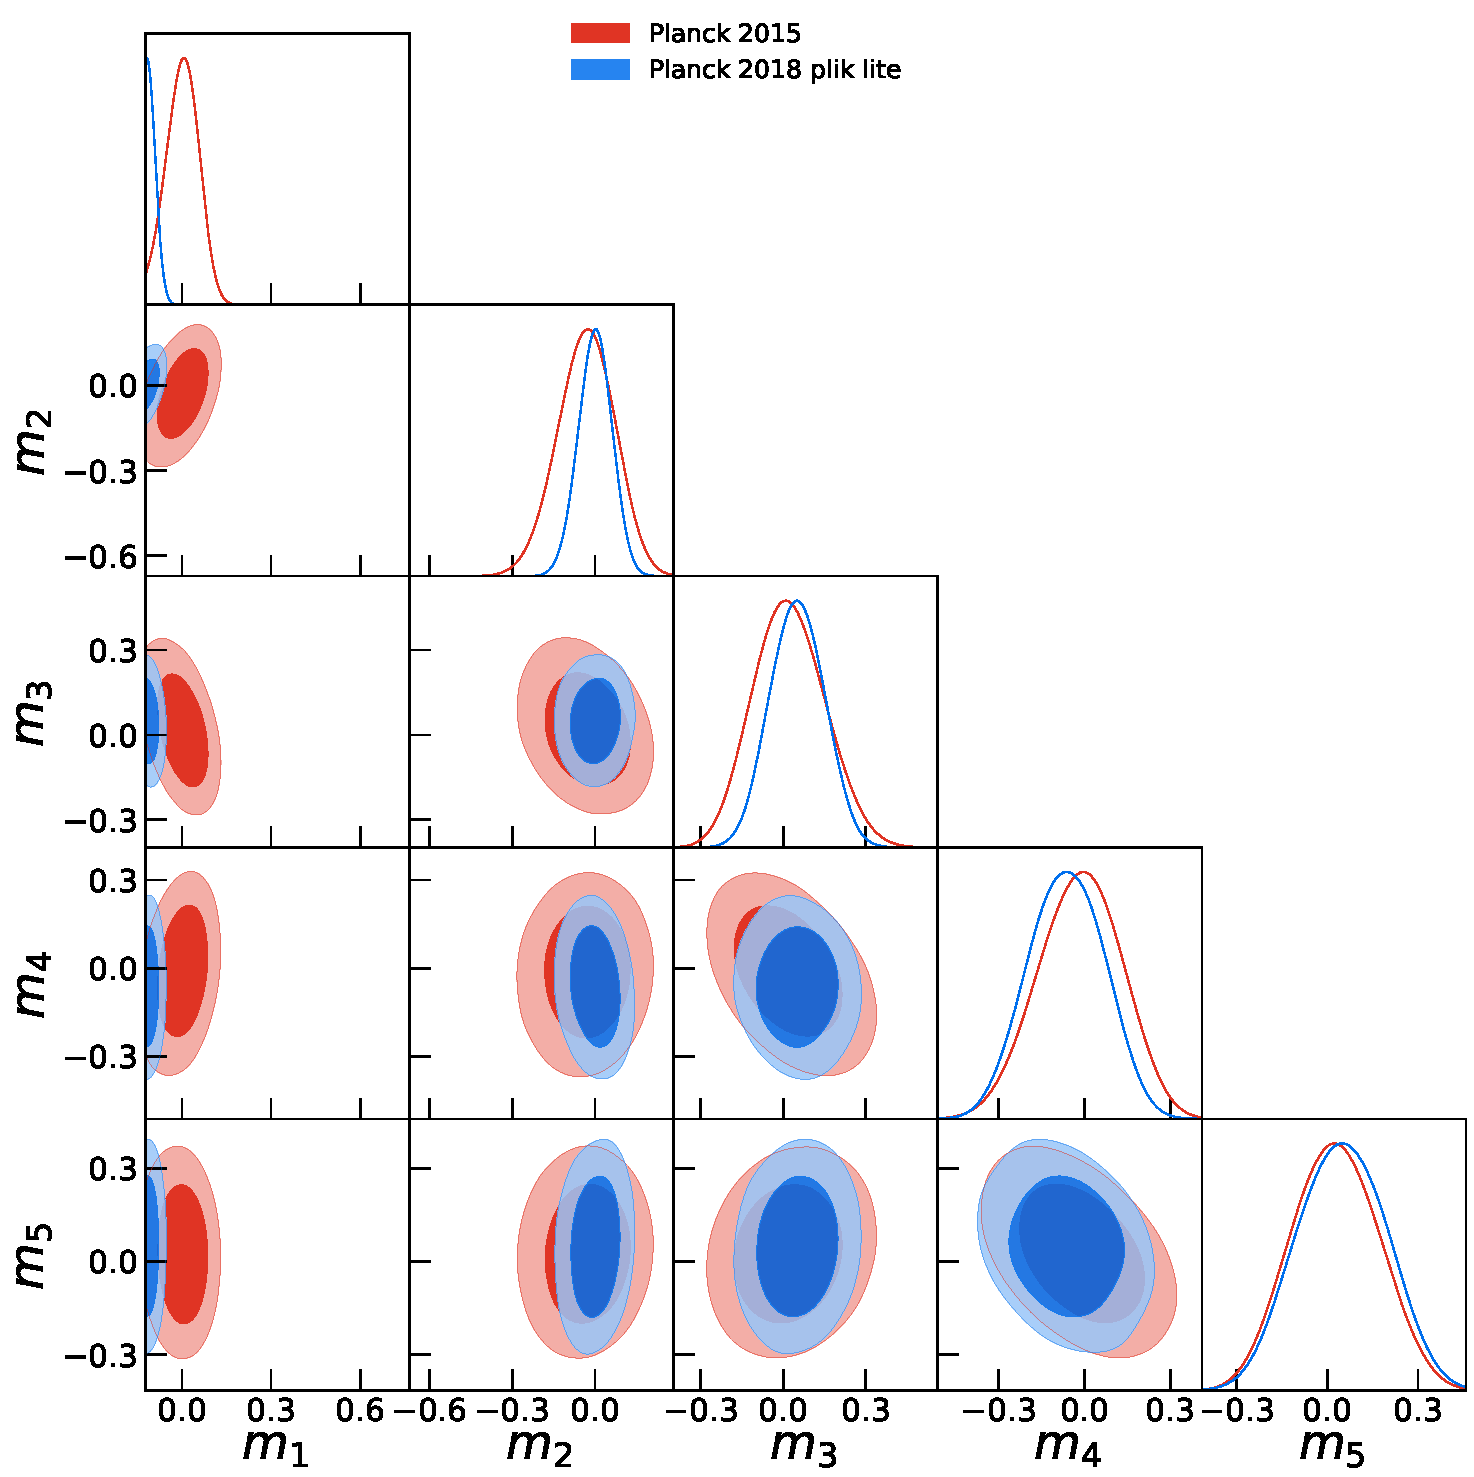
\includegraphics[width=0.7\textwidth]{results/pc_results/plot_mj_triangle_t18_r12_t19_t20_vs_pl18_pc_zmax30_pliklite.pdf}
\caption{Constraints from Planck data on the amplitudes of the five reionization principle components that describe all physical ionization models up to $z_{\rm max} = 30$. We show in red the Planck 2015 and the improved Planck 2018 contours in blue which uses the low-$\ell$ $EE$ likelihood \texttt{srollv2}. The 1D posterior distributions are shown on the diagonal and the 2D 68\% and 95\% C.L. regions in the $m_a-m_b$ planes in the lower triangle. The physicality priors on the ionization history used in this work are delineated by the box boundaries. [TODO: update legend]}
\label{fig:plot_mjs_2018_vs_2015}
\end{figure}

\end{widetext}

\begin{table}[b]
\centering
\caption{[Placeholder, need to fill in real numbers] PC chain means $\bar m_a$, standard deviations $\sigma(m_a)$, and correlation matrix $R_{ab}$.}
\label{tab:PC_stats}
\begin{tabular}{|r | r r@{\hskip 0.06in}|r r r r r|}
\hline
		
			  &  \multicolumn{1}{c}{$\bar m_a$} & \multicolumn{1}{c}{$\sigma(m_a)$}	 & \multicolumn{1}{|c}{$m_1$} & \multicolumn{1}{c}{$m_2$} & \multicolumn{1}{c}{$m_3$} & \multicolumn{1}{c}{$m_4$} & \multicolumn{1}{c|}{$m_5$} 
		\\ \hline
$m_1$ 
	& 0.002 & 0.053 & 1.000 & 0.450 & $-$0.432 & 0.273 & $-$0.073 \\ 
$m_2$ 
	& $-$0.030 &  0.101 & 0.450 & 1.000 & $-$0.262 & 0.055 & 0.072 \\ 
$m_3$ 
	& 0.019 &  0.128 & $-$0.432 & $-$0.262 &1.000 & $-$0.417 & 0.155 \\
$m_4$  
	& $-$0.012 & 0.143 &  0.273 & 0.055 & $-$0.417 & 1.000 & $-$0.428 \\ 
$m_5$ 
	& 0.026 & 0.143 & $-$0.073 & 0.072 & 0.155 & $-$0.428 & 1.000\\ \hline
\end{tabular}
\end{table}


\subsection{Comparison with Previous Results}

\begin{itemize}
    \item compare with Planck official results
    \item comment that Planck tau(15,30) constraints are too stringent (flex knots). Compare to ours. Point out why.
    \item{ Comments on priors (see below).}
    \item (*maybe in  another section): make a point that dz = 0.5 for tanh may not be sufficient for experiments after Planck. This was for higher tau, so transition happens at higher redshift. Now tau is much lower.
\end{itemize}


Recap our appendix from Planck 2015 on the issue of prior:
\begin{itemize}
    \item {describe tau prior issue raised by MB18: claimed that prior not flat in tau so bias PC; proposed to flatten by multiplying the inverse of prior point-by-point in the PC space; claim that this flattening removes a shift between tanh and PC results. }
    \item {summarize that we pointed it out the flaw in the logic in appendix of \cite{Heinrich:2018btc}.}
    \item{reproduce a few tests here: 1) tau12 posterior (no need to show again, point to appendix); 2) show prior boxes in m1-m2 plane (done in Fig.4) - repeat the length of lines of constant tau12 within the box describe the prior distribution. Make the point that though the line rises, the Planck data is more informative than priors in m1, m2 makes no impact on the posterior. However when inverting the prior, introduces a bias in tau.}
    \item{show test of explicitly constructing a prior that's locally flat in m1-m2, show posterior almost doesn't change. (only change is low-z enhancement, due to prior cut off at $z>6$. between our two priors, things don't change as much (might want to reproduce this result for this Planck 2018 results. And marius version too?}
    \item{inversion method should not be used on future dataset, since data is more informative than prior.}
\end{itemize}



\begin{figure}
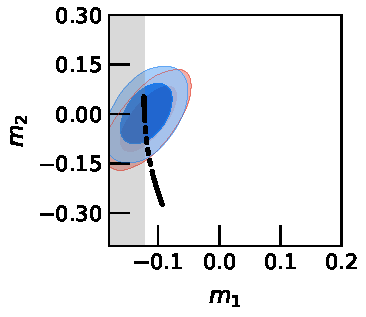
\includegraphics[width=0.4\textwidth]{results/pc_results/plot_m1_m2_pl18_pc_zmax30_pliklite_srollv2_vs_pl18_pc_zmax30_pliklite_wTauTrajectory.pdf}
\caption{The best-constrained $z_{\rm max} = 30$ PC plane, $m_1-m_2$. We compare Planck 2018 results with two different low-$\ell$ $EE$ likelihoods: the official \texttt{lowE} likelihood vs. the third-party released \texttt{srollv2} likelihood (zoomed-in from Fig.~\ref{fig:plot_mjs_2018_vs_2015}). [Comments on shift m1-m2 plane]. [TODO: Add Gaussian covariance, add legend, shrink x-axis]
}
\label{fig:plot_m1m2}
\end{figure}

\begin{figure}
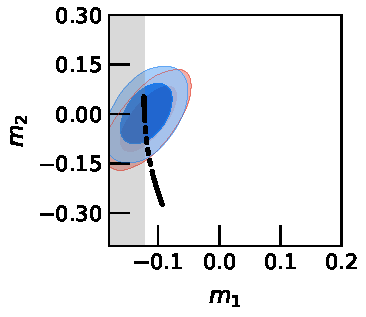
\includegraphics[width=0.4\textwidth]{results/pc_results/plot_m1_m2_pl18_pc_zmax30_pliklite_srollv2_vs_pl18_pc_zmax30_pliklite_wTauTrajectory.pdf}
\caption{[placeholder, maybe not] need m1-m2 plane for zmax = 30 using Planck 2018 vs 2015.
}
\label{fig:plot_m1m2}
\end{figure}

 
 \begin{figure}
          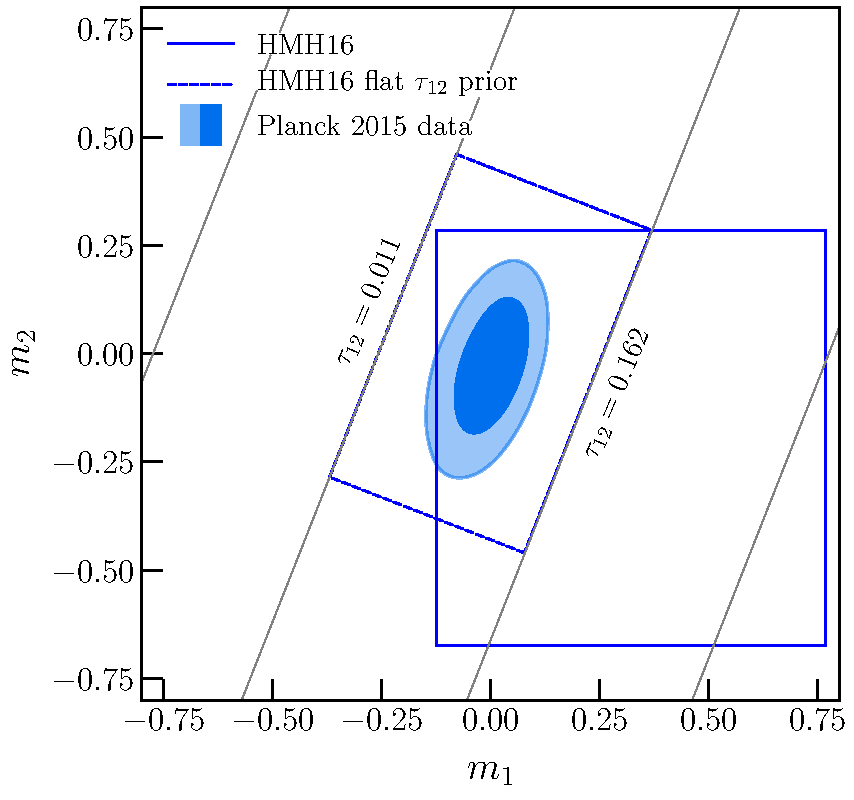
\includegraphics[width=0.9\columnwidth]{paper/plots/plot_rotated_box_flat_tau_prior_fac_0p8.pdf}
          \caption
          {[Placeholder right now (Planck 2015 plot)] Priors on the $m_1-m_2$ parameter space: the original HMH16 prior (inset square, solid lines) and a prior that is flat in
          both $\tau_{12}$ and $m_1-m_2$ (rotated rectangle, dashed lines) whose sides are aligned with lines of
          constant $\tau_{12}$ (light gray lines).   The HMH16 prior allows more parameter space at high vs low $\tau_{12}$ but this
          is not relevant since the data constraints (ellipses) exclude this region.  In the allowed region, the only difference is that the HMH16 prior clips the low $m_1$ edge of the allowed region due to physicality and the assumption that reionization occurs at
          $z\ge 6$. [add in text the comparison of priors, and how tau is not biased, and for KDE physical models determine the priors]}  \label{fig:prior_box}
\end{figure}


[Plot: add plot for tau(>z) contours for the 2 parameter model vs PC; direct integration first]

\begin{figure}[ht]
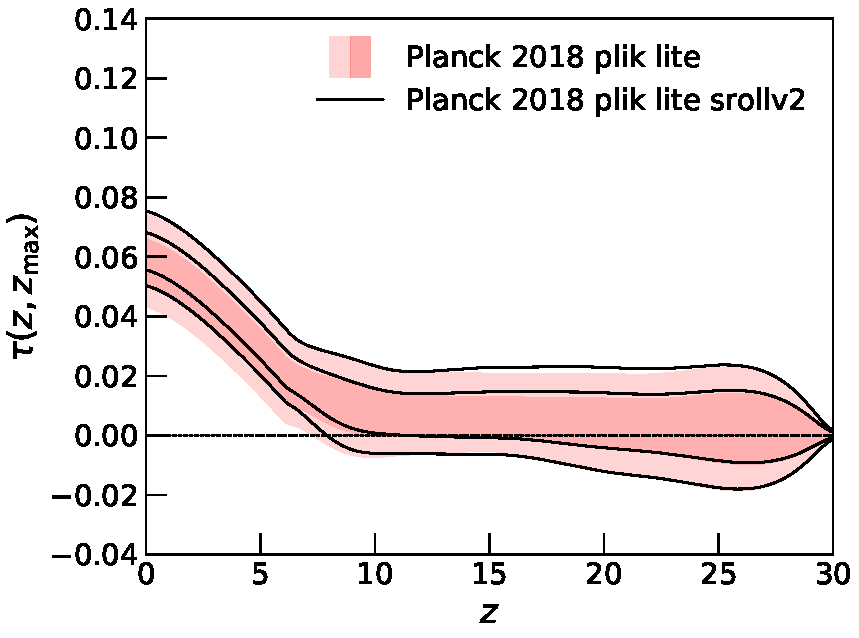
\includegraphics[width=0.45\textwidth]{results/direct_mcmc/pl18_plots_zmax30/plot_pub_tau_gtz_dz_0p1_pl18_pc_zmax30_pliklite_post_0930_and_pl18_pc_zmax30_pliklite_srollv2_0930.pdf}
\caption{[placeholder] PC chains for zmax = 30. Planck 2018 srollv2 likelihood vs Planck 2015).
}
\label{fig:}
\end{figure}

\begin{figure}[ht]
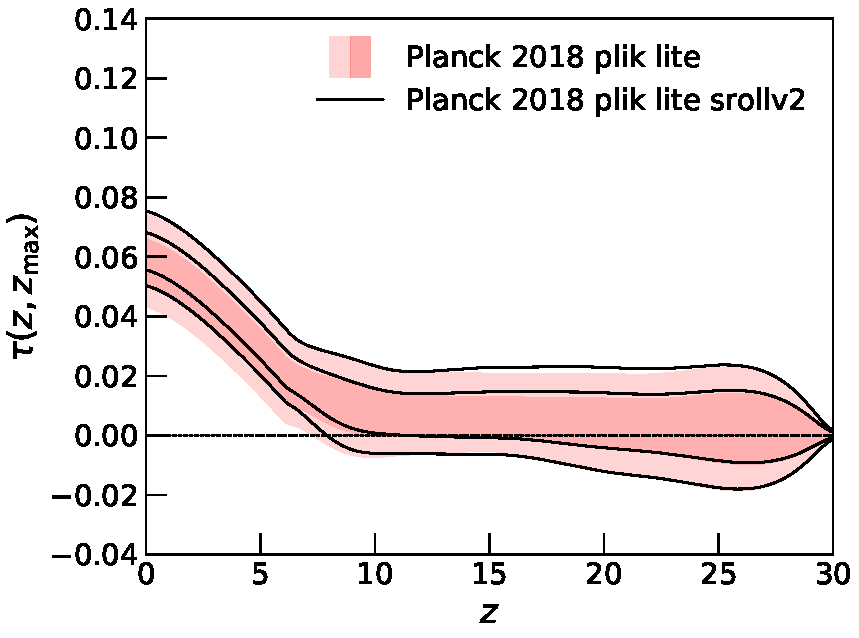
\includegraphics[width=0.45\textwidth]{results/direct_mcmc/pl18_plots_zmax30/plot_pub_tau_gtz_dz_0p1_pl18_pc_zmax30_pliklite_post_0930_and_pl18_pc_zmax30_pliklite_srollv2_0930.pdf}
\caption{PC chains for zmax = 30. Planck 2018 original lowE vs srollv2 likelihood (plik\_lite\_TTTEEE + lowl + simall\_EE vs plik\_lite\_TTTEEE + lowl + sroll2\_EE).
}
\label{fig:}
\end{figure}

\begin{figure}[ht]
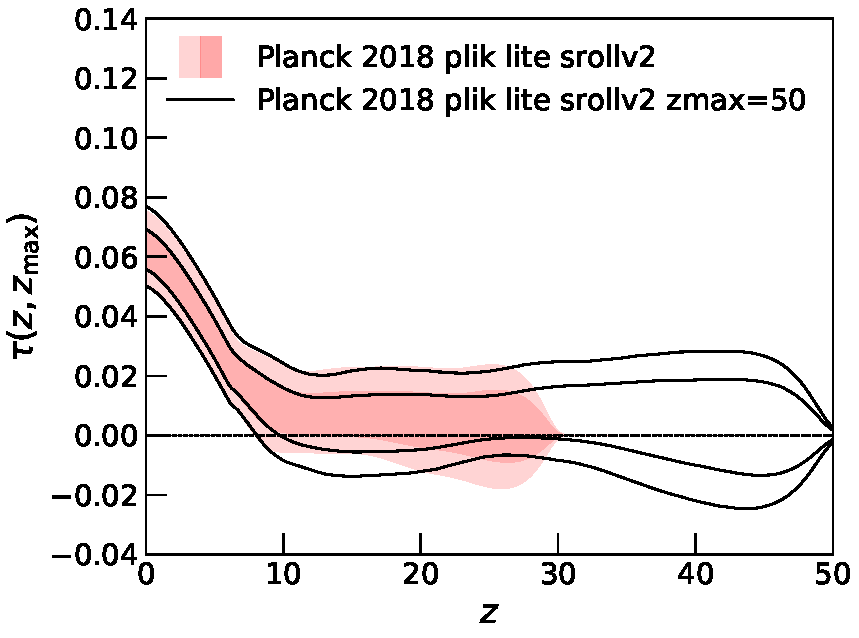
\includegraphics[width=0.45\textwidth]{results/direct_mcmc/pl18_plots_zmax30/plot_pub_tau_gtz_dz_0p1_pl18_pc_zmax30_pliklite_srollv2_0930_and_pl18_pc_zmax50_pliklite_srollv2.pdf}
\caption{Comparing zmax = 30 and 50 PC chains using Planck 2018 original lowE likelihood (plik\_lite\_TTTEEE + lowl + sroll2\_EE). Note that the zmax = 30 uses 5 PCs, whereas the zmax = 50 chains uses 7 PCs. .
}
\label{fig:}
\end{figure}

%Optional
\begin{figure}[ht]
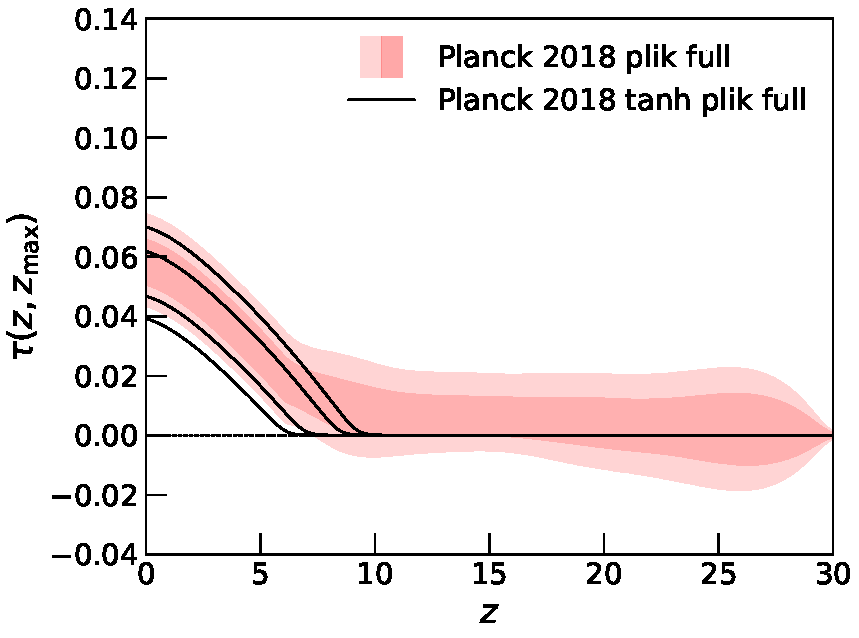
\includegraphics[width=0.5\textwidth]{results/direct_mcmc/pl18_plots_zmax30/plot_pub_tau_gtz_dz_0p1_pl18_pc_zmax30_plikfull_and_pl18_tanh_post_plikfull.pdf}
\caption{PC zmax = 30 vs tanh chains with plik\_full\_TTTEEE for the high-l likelihood.
}
\label{fig:}
\end{figure}


\begin{figure}
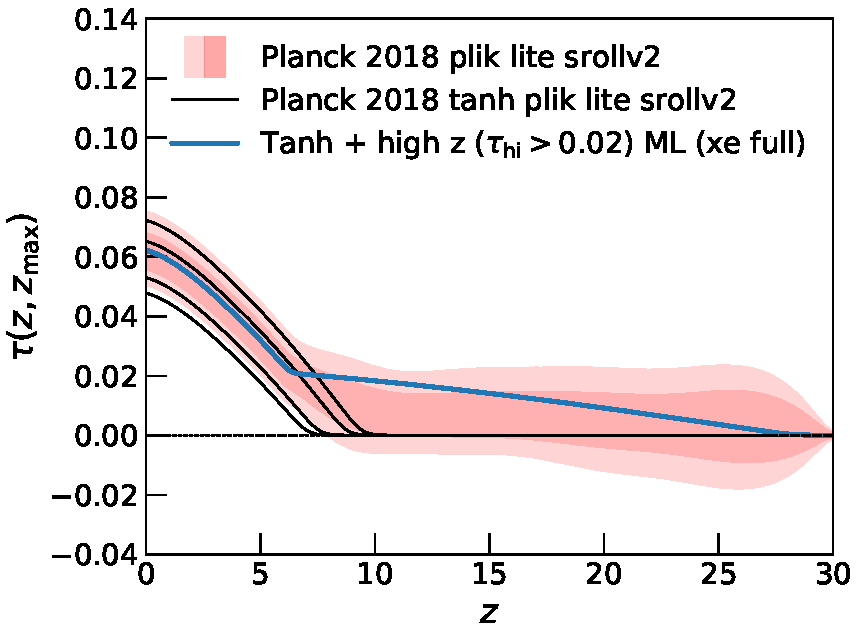
\includegraphics[width=0.40\textwidth]{plots/plot_tau_gtz.pdf}
\caption{...
}
\label{fig:}
\end{figure}


\begin{figure}
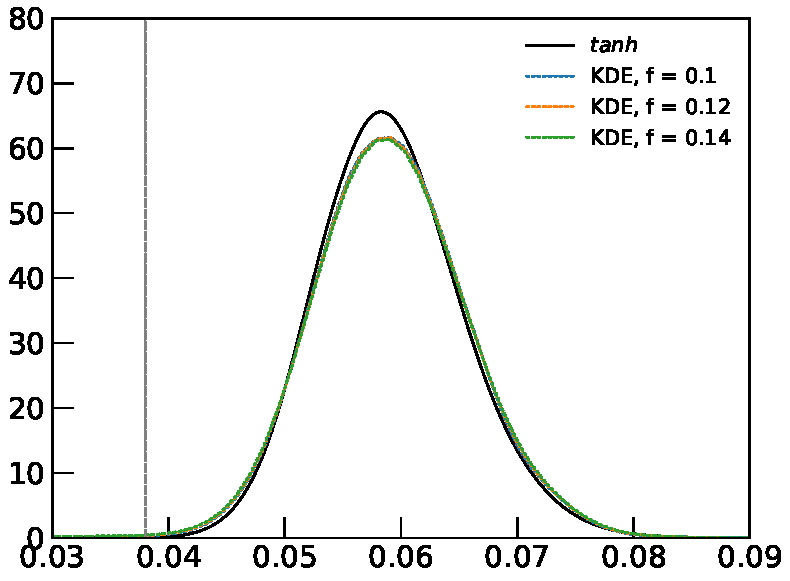
\includegraphics[width=0.40\textwidth]{plots/pl18_pc_zmax30_pliklite_srollv2_1015_tau_posterior_fraccov_1p0_burnin_10000_yes_norm_gaussian0p1_0p12_0p14.pdf}
\caption{...
}
\label{fig:}
\end{figure}



%%%%%%%%%%%%%%%%%%%%%%%%%%%%%%%%%%%%%%%%%%%%

\section{Effective Likelihood}
\label{sec:effective_likelihood}

\subsection{Code description}
\label{sec:code}

\subsection{Example 1: tanh model}
\label{sec:example1}

In Fig.~\ref{fig:reion_models}, we show the fiducial ionization history (thick blue) and contrast it with
the standard approach of CAMB (thin black) that takes hydrogen and singly ionized helium reionization to be given by
the tanh form
 \begin{equation}
x_e^{\rm true}(z) = \frac{1+f_{\rm He}}{2}\left\{  1+ \tanh\left[ \frac{y(z_*)-y(z)}{\Delta y} \right] \right\},
 \label{eqn:tanh}
 \end{equation}
 with $y(z)=(1+z)^{3/2}$, $\Delta y=(3/2)(1+z)^{1/2}\Delta z$, and $\Delta z = 0.5$.  We take here $z_*= 9.85$, corresponding the chain maximum likelihood (ML) model ($\tau = 0.0765$) from \S \ref{sec:MCMC},  for illustrative purposes.   Projected onto 5 PCs and resummed into $x_e(z)$, Eq.~(\ref{eq:mmutoxe}) yields a poor reconstruction of the ionization history itself.
 Nonetheless as we shall see in Fig.~\ref{fig:clee}, the PC decomposition provides an 
 excellent representation of the polarization power spectrum.
 

\subsection{Example 2: high-z model}
\label{sec:example2}
[rewording needed]
Our example is a two-step model 
 \bea
x_e^{\rm true}&(z)&\,= \frac{1+f_{\rm He} - \xemin}{2}\left\{  1+ \tanh\left[ \frac{y(z_{\rm re})-y(z)}{\Delta y} \right] \right\} \notag \\
&+& \frac{\xemin - x_e^{\rm rec}}{2}\left\{  1+ \tanh\left[ \frac{z_{\rm t}-z}{\Delta z_{2}} \right] \right\} + x_e^{\rm rec},
 \label{eqn:tanh_highz}
 \eea
where $y(z)=(1+z)^{3/2}$, $\Delta y=(3/2)(1+z)^{1/2}\Delta z_1$, with $\Delta z_1 = 0.25$ instead of the usual $\Delta z_1 = 0.5$,
to provide sharper distinctions between the two steps.
We choose the second step to have $z_{\rm t}=28$  and  $\Delta z_2 = 1.0$  to illustrate below
how the 5 PC analysis with $\zmax=30$ represents the same model.  Here $x_e^{\rm rec}$ is the ionization history from recombination only.
The canonical tanh model is essentially recovered in the limit $\xemin$ approaches the negligible $x_e^{\rm rec}$.  Therefore the double
step model adds a single parameter to control the high-$z$ ionization plateau for $z_{\rm re} \lesssim z \lesssim z_t$.   We show an example
of the two-step model in Fig.~\ref{fig:two_step_model}.


\begin{figure}
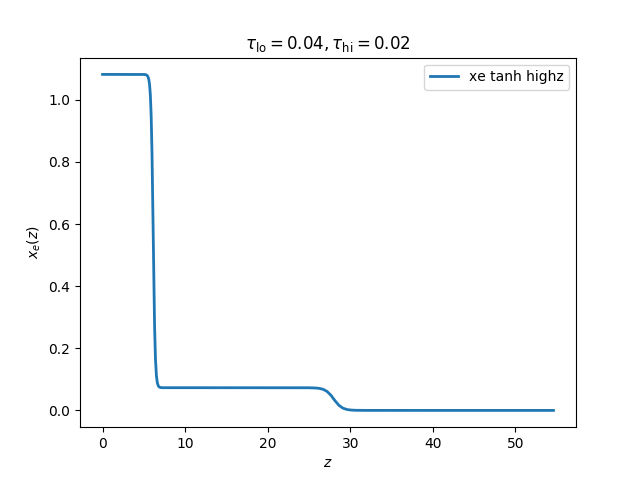
\includegraphics[width=0.5\textwidth]{results/cosmomc_kde/taulo_prior_test/plot_xez_taulo_0p04_tauhi_0p02.png}
\caption{Testing \taulo prior -- Full $x_e(z)$ of the model (\taulo, \tauhi) = (0.04, 0.02) shown in the Fig.~\ref{fig:taulo_prior_test_cl}. 
}
\label{fig:two_step_model}
\end{figure}

\begin{figure}
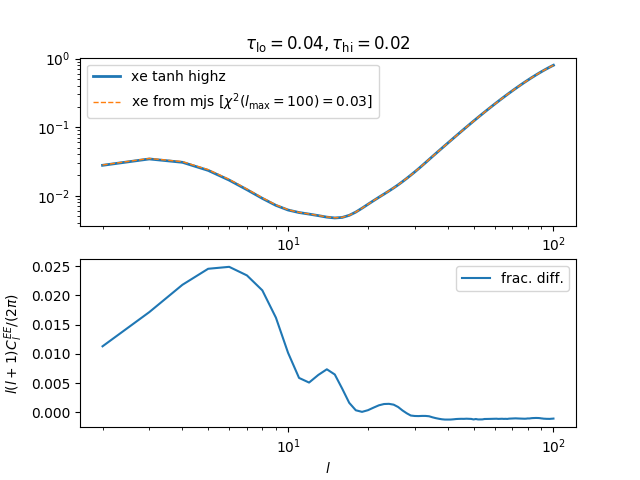
\includegraphics[width=0.5\textwidth]{results/cosmomc_kde/taulo_prior_test/plot_cls_taulo_0p04_tauhi_0p02.png}
\caption{Testing \taulo prior -- testing that \taulo $\geq$ 0.04 as \taulo prior is OK, by calculating $\chi^2$ between $C_l$ from full $x_e(z)$ vs PC decomposition of the model (\taulo, \tauhi) = (0.04, 0.02). 
The $\chi^2 = \sum_{2}^{l_{\rm max}} (\Delta C_l^{EE})^2 / \mathrm{Cov}_l = 0.03$ where $\mathrm{Cov}_l = 2 (C_l^{EE})^2/(2l+1)$. } 
\label{fig:taulo_prior_test_cl}
\end{figure}



\begin{figure}
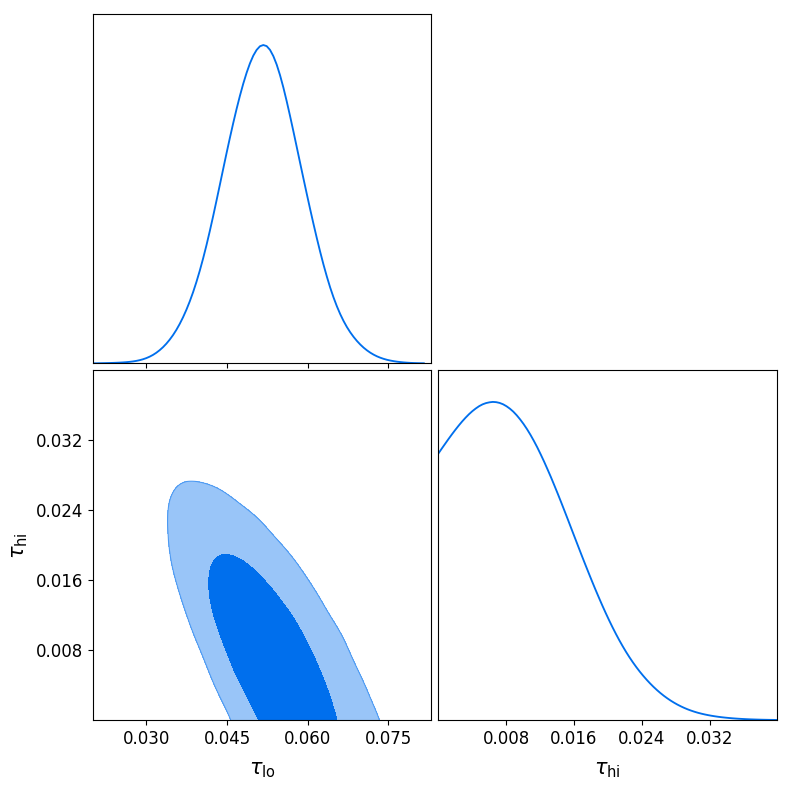
\includegraphics[width=0.5\textwidth]{results/direct_mcmc/two_parameter_model/tauhi_taulo_chains/pl18_tanh_highz_test2_run1_tri.png}
\caption{Direct MCMC chains of the two-parameter model with \tauhi and \taulo: triangle plot of \tauhi and \taulo. The marginalized 1D constraints are \taulo = $0.0516 \pm 0.0076$, \tauhi = $0.0100 \pm   0.0066$. The ML model is \taulo = 0.0543 and \tauhi = 0.0054 corresponding to $z_{\rm re} = 7.68$ and $x_{e, \mathrm{min}} = 0.021$.
}
\label{fig:two_parameter_model_2D_plot}
\end{figure}


\section{Conclusion}
\label{sec:conclusion}


\bibliography{rei.bib}

\appendix

\section{Outline (in progress)}

\begin{enumerate}
    \item{Intro}
        \begin{enumerate}
            \item 1st paragraph: CMB, reionization, why important
            \item discuss modeling of ionization history in CMB inference, tanh vs PCs (fail to capture high-z; PC captures complete parameter space), mention flex knots/other methods; cite previous PC works.
            \item give context about Planck final results; latest srollv2 likelihood, important to harness all information available, PC allows us to do that and turn into an effective likelihood.
            \item this is what we did: we obtain PC results for Planck 2018, and turn PC chains into a effective likelihood for ionization history: highlight key points like fast inference, entire model space up to zmax 30, code publicly available.
            \item we also compared to Planck official results, which is over stringent at high z, which gives additional motivations for using this likelihood; verified no hint of ionization at z>30; state any additional results.
            \item break down of sections.
        \end{enumerate}

	\item{Background}
		\begin{itemize}
			\item{Reionization Principal Components}	
			\item{Kernel Density Estimate}
		\end{itemize}
	\item{Planck 2018 PC results:\\
		- can discuss discrepancy here on high-redshift tau($>$15) constraints.\\
		- compare with our own 2015 PC results
		- zmax = 30 vs 50}
	\item{Effective Likelihood}
		\begin{itemize}
			\item{Code Description}
			\item{Examples - one and two parameter models}
		\end{itemize}
	\item{Discussion}
		
\end{enumerate}


\end{document}
